\documentclass[lettersize,journal]{IEEEtran} %这一行的作用是设置论文的格式,letterpaper表示纸张大小为美国信纸,journal表示论文类型为期刊论文,IEEEtran表示论文的格式为IEEEtran
\usepackage{amsmath,amsfonts} %这两个包分别是数学公式和数学字体的宏包
\usepackage{algorithm}
\usepackage{algpseudocode}
% \usepackage{algorithmic} %这个包是算法的宏包
\usepackage{array} %这个包是表格和数组的宏包
% \usepackage[caption=false,font=normalsize,labelfont=sf,textfont=sf]{subfig} %这个包是子图的宏包,它可以让你在一个图形环境中放置多个图形,可以对子图进行编号,可以对子图进行交叉引用,可以对子图进行标题设置
\usepackage{textcomp} %这个包是对文本模式下的符号进行扩展的宏包
\usepackage{stfloats} %这个包是控制双栏浮动图形和表格的宏包
\usepackage{url} %这个包是对网址进行扩展的宏包
\usepackage{verbatim} %这个包是对抄录环境进行扩展的宏包
\usepackage{graphicx} %这个包是对图形进行扩展的宏包
\usepackage{subcaption}
\usepackage{multirow}
\hyphenation{op-tical net-works semi-conduc-tor IEEE-Xplore} %这一行的作用是设置英文连字符,可以防止英文单词在换行时过长
\def\BibTeX{{\rm B\kern-.05em{\sc i\kern-.025em b}\kern-.08em
    T\kern-.1667em\lower.7ex\hbox{E}\kern-.125emX}} %这一行的作用是定义BibTeX的标志,这个标志在参考文献中会用到
\usepackage{balance} %这个包是平衡双栏文档最后一页的双栏高度的宏包



\begin{document} %这一行的作用是开始论文的正文部分
\title{GraphCPP: A Data-Driven Graph Processing System for Concurrent Point-to-Point Queries} %这一行的作用是设置论文的标题
\author{IEEE Publication Technology Department %这一行的作用是设置论文的作者
\thanks{Manuscript created October, 2020; This work was developed by the IEEE Publication Technology Department. This work is distributed under the \LaTeX \ Project Public License (LPPL) ( http://www.latex-project.org/ ) version 1.3. A copy of the LPPL, version 1.3, is included in the base \LaTeX \ documentation of all distributions of \LaTeX \ released 2003/12/01 or later. The opinions expressed here are entirely that of the author. No warranty is expressed or implied. User assumes all risk.}} %这一行的作用是设置论文的作者的单位和邮箱,这里的\thanks是设置脚注的命令

\markboth{Journal of \LaTeX\ Class Files,~Vol.~18, No.~9, September~2023}%这一行的作用是设置论文的页眉
{How to Use the IEEEtran \LaTeX \ Templates} 

\maketitle %它和title的区别是,title只是设置论文的标题,而maketitle是使论文的标题和作者的信息生效

\graphicspath{{E:/华科实验室论文/MyDocument/并发点对点查询/论文草稿/picture/}}


\begin{abstract} %这一行的作用是设置论文的摘要
With the widespread adoption of graph processing technology in fields such as map navigation and network analysis, a considerable number of point-to-point query tasks run concurrently on the same underlying graph, imposing a high demand on the throughput of graph query systems. However, existing graph processing systems either focus on optimizing the speed of individual point-to-point queries, neglecting the throughput of concurrent queries, or follow the concurrent execution approach of point-to-all algorithms, overlooking the optimization potential of point-to-point algorithms. Due to redundant data access overhead and computational expenses, existing solutions exhibit poor overall throughput when executing concurrent point-to-point queries.

This paper introduces GraphCPP, the first graph traversal system designed for concurrent execution of point-to-point query tasks. It enhances the throughput of concurrent query tasks through data access sharing and hot path computation sharing. GraphCPP is novel in two ways. Firstly, based on the observation that traversal paths for different query tasks overlap significantly, GraphCPP proposes a data-driven caching execution mechanism.  Through fine-grained graph chunk scheduling, this mechanism enables data sharing among concurrent tasks, thereby enhancing data access efficiency. Secondly, recognizing the frequent computation of the same hot vertices and paths by distinct tasks, GraphCPP proposes a dual-level computation sharing mechanism. This mechanism accelerates the convergence of new queries by sharing computed values of hot vertices and paths. In our evaluation on datasets such as xx, we compare GraphCPP with state-of-the-art point-to-point query systems and concurrent graph processingsystems. The results demonstrate that GraphCPP incurs only xx preprocessing overhead and xx storage overhead, achieving a throughput improvement of xx-xx times compared to SGraph, Tripoline, Pnp, and Glign.
  
\end{abstract}



\begin{IEEEkeywords}
graph process, point-to-point queries, concurrent jobs, data access similarity, computational similarity.
\end{IEEEkeywords}


\section{Introduction}
\IEEEPARstart{A} significant number of concurrent point-to-point query tasks are commonly executed on the same underlying graph. For instance, in logistics and transportation, Google Maps [xx] identifies the optimal route between two locations. In social network analysis, Facebook [x] recommends potential friends to users by exploring the relationship chain between two users. In financial risk analysis, Alipay [x] analyzes how risk spreads from one entity to another. These popular applications highlight the demand for executing large-scale concurrent point-to-point queries on the same underlying graph. However, existing solutions for point-to-point queries [xxxx] primarily focus on accelerating the efficiency of individual queries while neglecting optimization for concurrent queries. To achieve the efficient execution of concurrent point-to-point query tasks, two key challenges need to be addressed.


Firstly, executing concurrent point-to-point query tasks on the same underlying graph without considering data access similarity leads to redundant access to overlapping data. Specifically, different query tasks start from distinct origins and eventually reach their respective destinations. There is a significant overlap in their traversal paths. However, as the overlapping portions of data accessed by different query tasks vary, and they traverse overlapping graph data along different paths. Therefore, existing query systems adopt a conservative strategy, assigning each task to access the data it requires independently. This means that the data access for each task is entirely isolated, even if their traversal paths highly overlap. For example, if the path of one query is a subset of the path of another query, the overlapping data needs to be loaded redundantly, preventing the benefits of reusing data in the cache.

Secondly, in addition to redundant access, different query tasks also face the challenge of recalculating path values for popular paths. As graph data often exhibits a power-law distribution, a small number of popular vertices frequently appear in the optimal paths of different queries. Due to the lack of computation sharing among different query tasks, they redundantly compute the hot paths connecting popular vertices. Moreover, popular vertices often correspond to high-degree vertices with numerous neighboring vertices, and the repetitive traversal of these vertices results in an explosive growth in computation costs. Some existing systems have attempted to implement computation sharing through global indexing [xxxx], but the efficiency and accuracy of computation sharing are limited by the expensive computational, storage, and update costs.

To address the challenges mentioned above, this paper proposes a data-driven concurrent point-to-point query system called GraphCPP. It enhances the throughput of concurrent point-to-point query systems through data sharing and computation sharing mechanisms.

In GraphCPP, we firstly introduce a data-driven caching execution mechanism that transforms the traditional $task \rightarrow data$ scheduling approach into a $data \rightarrow task$ scheduling approach, thereby enabling the sharing of overlapping graph structure data among multiple tasks. Under this execution mechanism, GraphCPP first determines the scheduling order of data: it logically partitions graph structure data into fine-grained chunks at the LLC level. Subsequently, it associates query tasks with the relevant graph chunks based on the graph block where the active vertices of the query tasks reside. The higher the number of associated tasks, the higher the priority for scheduling that chunk. As the set of active vertices changes in each round, and the number of associated tasks for shared chunks needs updating in each round, GraphCPP adopts an associated task-triggering mechanism to achieve $data \rightarrow task$ scheduling. After loading the graph chunks into the LLC in priority order, the system utilizes the associated information obtained in each round to trigger the batch execution of associated tasks for the current chunk, efficiently accessing shared data.

Besides, GraphCPP proposes a dual-level computation sharing mechanism including global indexing and core subgraph indexing. It designates vertices with a substantial number of connecting edges in the graph as hot vertices and the paths between hot vertices as hot paths. Although the proportion of hot vertices and hot paths is small, they occur frequently in traversal paths to different query tasks. The dual-level computation sharing mechanism achieves the first level of computation sharing through global indexing. The global index maintains a small set of hot vertices and their index values to other vertices. These hot vertices act as intermediary nodes for different query paths, providing prunable path values for the majority of queries. Through the core subgraph mechanism, the second level of computation sharing is realized. The core subgraph primarily maintains hot paths connecting hot vertices in the graph. It is essential to note that the number of hot vertices in the core subgraph is an order of magnitude larger than that in the global index. Specifically, it first filters hot vertices with high degrees from the original graph data. Subsequently, it traverses hot paths between these vertices, assigning the path values as weights to the edges between pairs of hot vertices. During the querying process, the core subgraph plays a role similar to that of a high-speed highway network. Utilizing it allows traversal from one hot vertex to another, akin to entering a highway at a hot vertex and swiftly reaching other high-speed stations ($hot~vertices$) through the fast lanes ($hot~paths$) on the highway network. The dual-level computation sharing mechanism in GraphCPP mitigates redundant computations.

Lastly, GraphCPP further enhances the performance of concurrent queries by predicting the traversal paths of different query tasks and driving the batch execution of highly overlapping similar query tasks.

This paper makes the following contributions:
\begin{enumerate}
  \item{We analyze the performance bottlenecks of existing graph processing systems when handling concurrent point-to-point query tasks and propose leveraging the similarities in data access and computation among concurrent tasks to enhance throughput.}
  \item{We develop GraphCPP, a dynamic data-driven concurrent processing system for point-to-point queries. It achieves data sharing and computation sharing among concurrent tasks and introduces a strategy for batch execution of similar tasks.}
  \item{We compare GraphCPP with three state-of-the-art point-to-point query systems, namely XXXXXX, using a workload that includes x real-world graphs and x applications. Our experiments demonstrate that, on average, GraphCPP outperforms others, achieving xx times, xxx times, and xxx times improvement compared to XXX, XXX, and XXX, respectively.}
\end{enumerate}

\section{BACKGROUND AND MOTIVATION}
Most existing solutions [xxx] are primarily focused on accelerating the speed of individual queries. However, in practical scenarios, there is a significant number of graph query tasks concurrently running on the same underlying graph. For instance, statistics from CAGIS[xx] indicate that location service open platforms constructed by companies such as Baidu Maps[xx], Amap[xx], Tencent Maps[xx], and Huawei Maps[xx] receive a daily average of up to 160 billion location service requests. The substantial demand for concurrent point-to-point queries poses a high requirement for the throughput of graph traversal systems. However, as illustrated in table 1, we demonstrate that existing systems exhibit low throughput when handling large-scale concurrent queries. The root cause of this undesirable outcome is the significant redundancy in data access and computation among concurrent tasks. To qualitatively analyze the aforementioned issues, we conducted performance evaluations on parallel point-to-point queries using XXXXX (machine configuration), selecting XXXXX (the current best solution) on XXXXX (graph dataset).

\begin{figure}[!t]
    \centering
    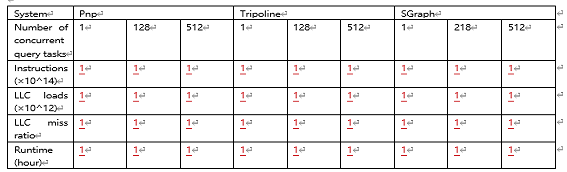
\includegraphics[width=\columnwidth]{system_compare.png}
    \caption{Your caption here}
    \label{fig:system_compare}
  \end{figure}


\subsection{Preliminaries}
Definition 1: ($Graph$) We use $G=(V,E)$ to denote a directed graph, where $V$ is the set of vertices, and $E$ is the set of directed edges formed by vertices in $V$ (for undirected graphs, edges can be split into two directed edges with different directions). We use $|V|$ and $|E|$ to represent the number of vertices and edges, respectively.

Definition 2: ($Graph~Partition$) We use $P_i=(V_{P_i},E_{P_i})$ to denote the $i_{th}  $ graph partition of a directed graph, where $V_{P_i}$ represents the set of vertices in the graph partition, and $E_{P_i}$ is the set of directed edges composed of vertices in $V_{P_i}$. In a distributed system, different machine-specific graph partitions $P_i$ are distinct. We partition the graph using edge cuts, where the same vertex may appear on different computing nodes, but there is only one primary vertex, while the others are mirror vertices.

Definition 3: ($Point \text{-} to \text{-} Point~Quer$y) We use $q_i=(s_i,d_i)$ to denote the query corresponding to task $i$, where $s_i$ and $d_i$ represent the source and destination vertices of $q_i$, respectively. If the execution of the point-to-point query algorithm on the graph yields a convergent path for $q_i$, this path is referred to as the optimal path between $s_i$ and $d_i$.

Definition 4: ($Bounds$) In mainstream point-to-point query systems, a pruning-based query strategy is widely adopted, where $bounds$ provide conservative pruning values. Specifically, $bounds$ can be further categorized into $upper~bounds$ ($UB$) and $lower~bounds$ ($LB$). $UB$ represents the current known optimal path value from the source to the destination vertex, while $LB$ signifies a conservative predicted path value from the current vertex $v$ to the destination vertex, with the predicted $LB$ being less than or equal to the actual optimal path value from vertex $v$ to the destination vertex. Following the triangle inequality on the graph, if the value of a path is greater than $UB$ or exceeds $UB$ when adding the value of $LB$, the path is definitely worse than existing paths and needs to be pruned. The values of upper and lower $bounds$ need indexing to be derived, essentially constituting a form of computation sharing.

Definition 5: ($Core~Subgraph$) We use $G_{core}=(V_{hot},E_{hot},Index_{hot})$ to represent the $core~subgraph$, where $V_{hot}$ is the set of $hot~vertices$ , $E_{hot}$ abstracts the $hot~paths$ between vertices in $V_{hot}$ as edges, and $Index_{hot}$ represents the path values corresponding to $E_{hot}$. A $hot~vertex$ refers to a vertex in a graph with a significant number of edges. A $hot~path$ is defined as the optimal path between two $hot~vertices$. A $hot~index$ denotes the path value of a $hot~path$.

Definition 6: ($Index$) The $index$ records the optimal query path values between vertex pairs. GraphCPP sorts vertices by degree, selecting $k+m$ vertices with the highest degrees. Note that, values for $k$ and $m$ are generally user-determined, with $k$ usually set to 16, and $m$ typically one order of magnitude larger than $k$. The first $k$ vertices serve as $global~vertices$, while the remaining vertices function as $core~subgraph~vertices$. The $global~index$ records optimal query path values to all vertices in the graph. The $core~subgraph~index$ only records query path values between hot vertices in the subgraph.

\begin{figure}[!t]
    \centering
  
    \begin{subfigure}{0.3\columnwidth}
      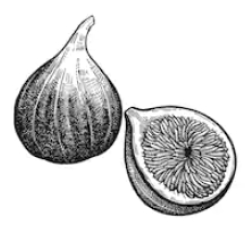
\includegraphics[width=\linewidth]{fig1.png}
      \caption{Caption for Subfigure 1}
      \label{fig:subfig1}
    \end{subfigure}
    \hfill
    \begin{subfigure}{0.3\columnwidth}
      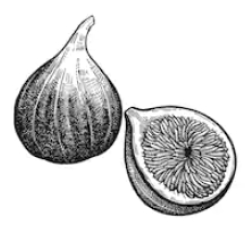
\includegraphics[width=\linewidth]{fig1.png}
      \caption{Caption for Subfigure 2}
      \label{fig:subfig2}
    \end{subfigure}
    \hfill
    \begin{subfigure}{0.3\columnwidth}
      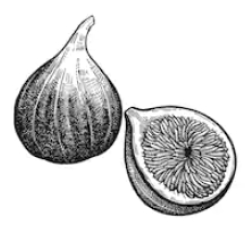
\includegraphics[width=\linewidth]{fig1.png}
      \caption{Caption for Subfigure 3}
      \label{fig:subfig3}
    \end{subfigure}
  
    \medskip
  
    \begin{subfigure}{0.3\columnwidth}
      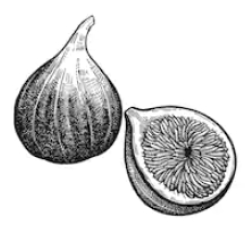
\includegraphics[width=\linewidth]{fig1.png}
      \caption{Caption for Subfigure 4}
      \label{fig:subfig4}
    \end{subfigure}
    \hfill
    \begin{subfigure}{0.3\columnwidth}
      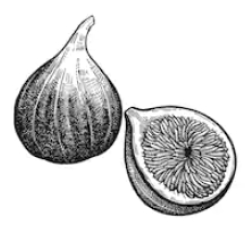
\includegraphics[width=\linewidth]{fig1.png}
      \caption{Caption for Subfigure 5}
      \label{fig:subfig5}
    \end{subfigure}
    \hfill
    \begin{subfigure}{0.3\columnwidth}
      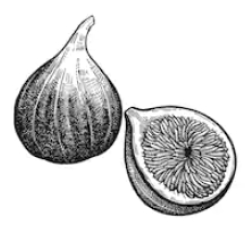
\includegraphics[width=\linewidth]{fig1.png}
      \caption{Caption for Subfigure 6}
      \label{fig:subfig6}
    \end{subfigure}
  
    \caption{Overall caption for the figure}
    \label{fig:overall}
  \end{figure}
  
  

\subsection{Performance Bottlenecks in Concurrent Point-to-Point Query Tasks}
In this section, we have implemented the concurrent version of the existing linear pairwise query system and the pairwise version of the existing concurrent graph computing system. Our objective is to quantitatively elucidate the performance bottlenecks of current concurrent pairwise query solutions.

{\bf{The redundant data access overhead of concurrent tasks is evident.}} We observe that when concurrent pairwise query tasks execute graph traversal on the same underlying graph, a significant portion of their traversal paths exhibits clear data access similarities. As shown in Figure 3x, our data indicates that there is a substantial overlap in data access among concurrent tasks, with a higher overlap ratio for similar tasks (more details are provided in Section xx). However, in the traditional $task \rightarrow data$ scheduling mode, different tasks independently execute queries, leading to competition for limited cache space to store their respective graph data chunks, even if these data chunks are identical. This results in severe cache thrashing and a reduction in the performance of processing concurrent pairwise queries. Table 1 illustrates that, with an increase in the number of concurrent tasks, the cache miss rate for query tasks sharply rises. Although the overall performance of concurrent execution surpasses linear execution, the average query time per task significantly increases with the growing number of query tasks due to the mentioned redundant data access overhead. It is essential to note that the total execution time in the concurrent mode is the maximum among the execution times of these tasks, while in the sequential mode, it is the sum of all task execution times.


{\bf{Redundant Computational Overhead of Concurrent Tasks.}} Unlike point-to-all queries, point-to-point query algorithms employ a targeted traversal strategy, significantly narrowing down the query scope. This focused exploration is a result of the algorithm's inherent selectivity. Given the power-law distribution characteristics of graph data, a significant portion of traversal paths in point-to-point queries involves hot vertices. While hot vertices make up only a small fraction of the total vertices (XX\%), they are prevalent in the traversal paths of many tasks (XX\%). Furthermore, the proportion of hot vertices in graph data marked by higher levels of sharing is even more pronounced. This suggests that various query tasks redundantly calculate hot paths between hot vertices, revealing computational similarities among concurrent tasks. Over a graph snapshot period, computational results for identical vertex pairs remain consistent, indicating significant redundancy in computational efforts across concurrent tasks. Additionally, due to the frequent possession of numerous outgoing and incoming edges by hot vertices, the computational overhead they introduce far exceeds that of ordinary vertices.

Some existing solutions utilize a global indexing mechanism [x] to achieve computational sharing associated with global vertices. However, the global indexing mechanism has inherent flaws. {\bf{Flaw 1}}: The global index requires recording path values between hot vertices and regular vertices. In large-scale graphs, the computational and storage costs of establishing the index can be substantial, as depicted in Figures 3 and 4, where the costs increase proportionally with the number of global index vertices. {\bf{Flaw 2}}: In point-to-point queries on streaming graphs, each round of graph updates introduces new edges and edge deletions. The global index needs to dynamically update the index relationships between high-degree vertices and every vertex based on the latest graph snapshot. This implies that any update to the streaming graph will impact all vertex indices, as illustrated in Figure 5, where a small number of graph updates lead to extensive updates in the global index. {\bf{Flaw 3}}: Different datasets have different data distribution patterns, making it challenging to choose an appropriate number of index vertices to balance the efficiency of computational sharing and the overhead of the index itself. As shown in Figure 6, selecting the same number of index vertices on different datasets results in significant variations in inherent costs and the effectiveness of computational sharing. In summary, the global indexing mechanism incurs expensive costs, and the fluctuation in required costs for different datasets is considerable. Therefore, existing systems often conservatively choose the number of global indices (e.g., 16 vertices in Tripoline\cite{tripoline} and SGraph\cite{sgraph}) to avoid excessive costs. However, this also limits the coverage range of global indices, preventing efficient computational sharing.


\subsection{Our Motivation}
Inspired by the observations mentioned above, we derive the following insights:

{\bf{Observation 1}}: A significant portion of traversal paths in different query tasks displays substantial overlap, indicating a similarity in data access patterns. However, existing solutions fall short in concurrently supporting point-to-point queries and facilitating data sharing among tasks, resulting in redundant data access. This observation motivates the development of an efficient, fine-grained data-sharing mechanism. By allowing various tasks to share access to the same data at different times, this mechanism aims to reduce data access costs and enhance the throughput of concurrent queries.

{\bf{Observation 2}}: The core subgraph, consisting of hot vertices and paths in the original graph, is frequently traversed by various tasks, highlighting computational similarity among different query tasks. Existing graph traversal systems either neglect computational similarity [xx pnp] or employ a costly global indexing mechanism [xx Tripoline], limiting the effectiveness of computational sharing. This observation inspires the creation of a lightweight, dual-layered indexing mechanism to share computational results of overlapping hot paths across different query tasks. 

\section{GraphCPP Overview}

\subsection{System Architecture}
To enhance the efficiency of concurrent point-to-point queries, we introduce GraphCPP, a meticulously designed, data-driven system tailored for concurrent query tasks. Developed after a thorough examination of the computational intricacies inherent in such queries, GraphCPP aims to achieve data and computation sharing among concurrent point-to-point tasks. As depicted in the figure below, GraphCPP incorporates an efficient data-driven caching execution mechanism, leveraging data similarity among concurrent tasks to facilitate shared access to overlapping data. Additionally, it introduces a dual-level computation sharing mechanism, enabling computations for identical hot vertices and paths to be shared across different query tasks. Furthermore, GraphCPP employs path prediction for various queries, promoting the bulk execution of similar queries with overlapping paths and maximizing the utilization of data similarity. 

\begin{figure}[!t]
    \centering
    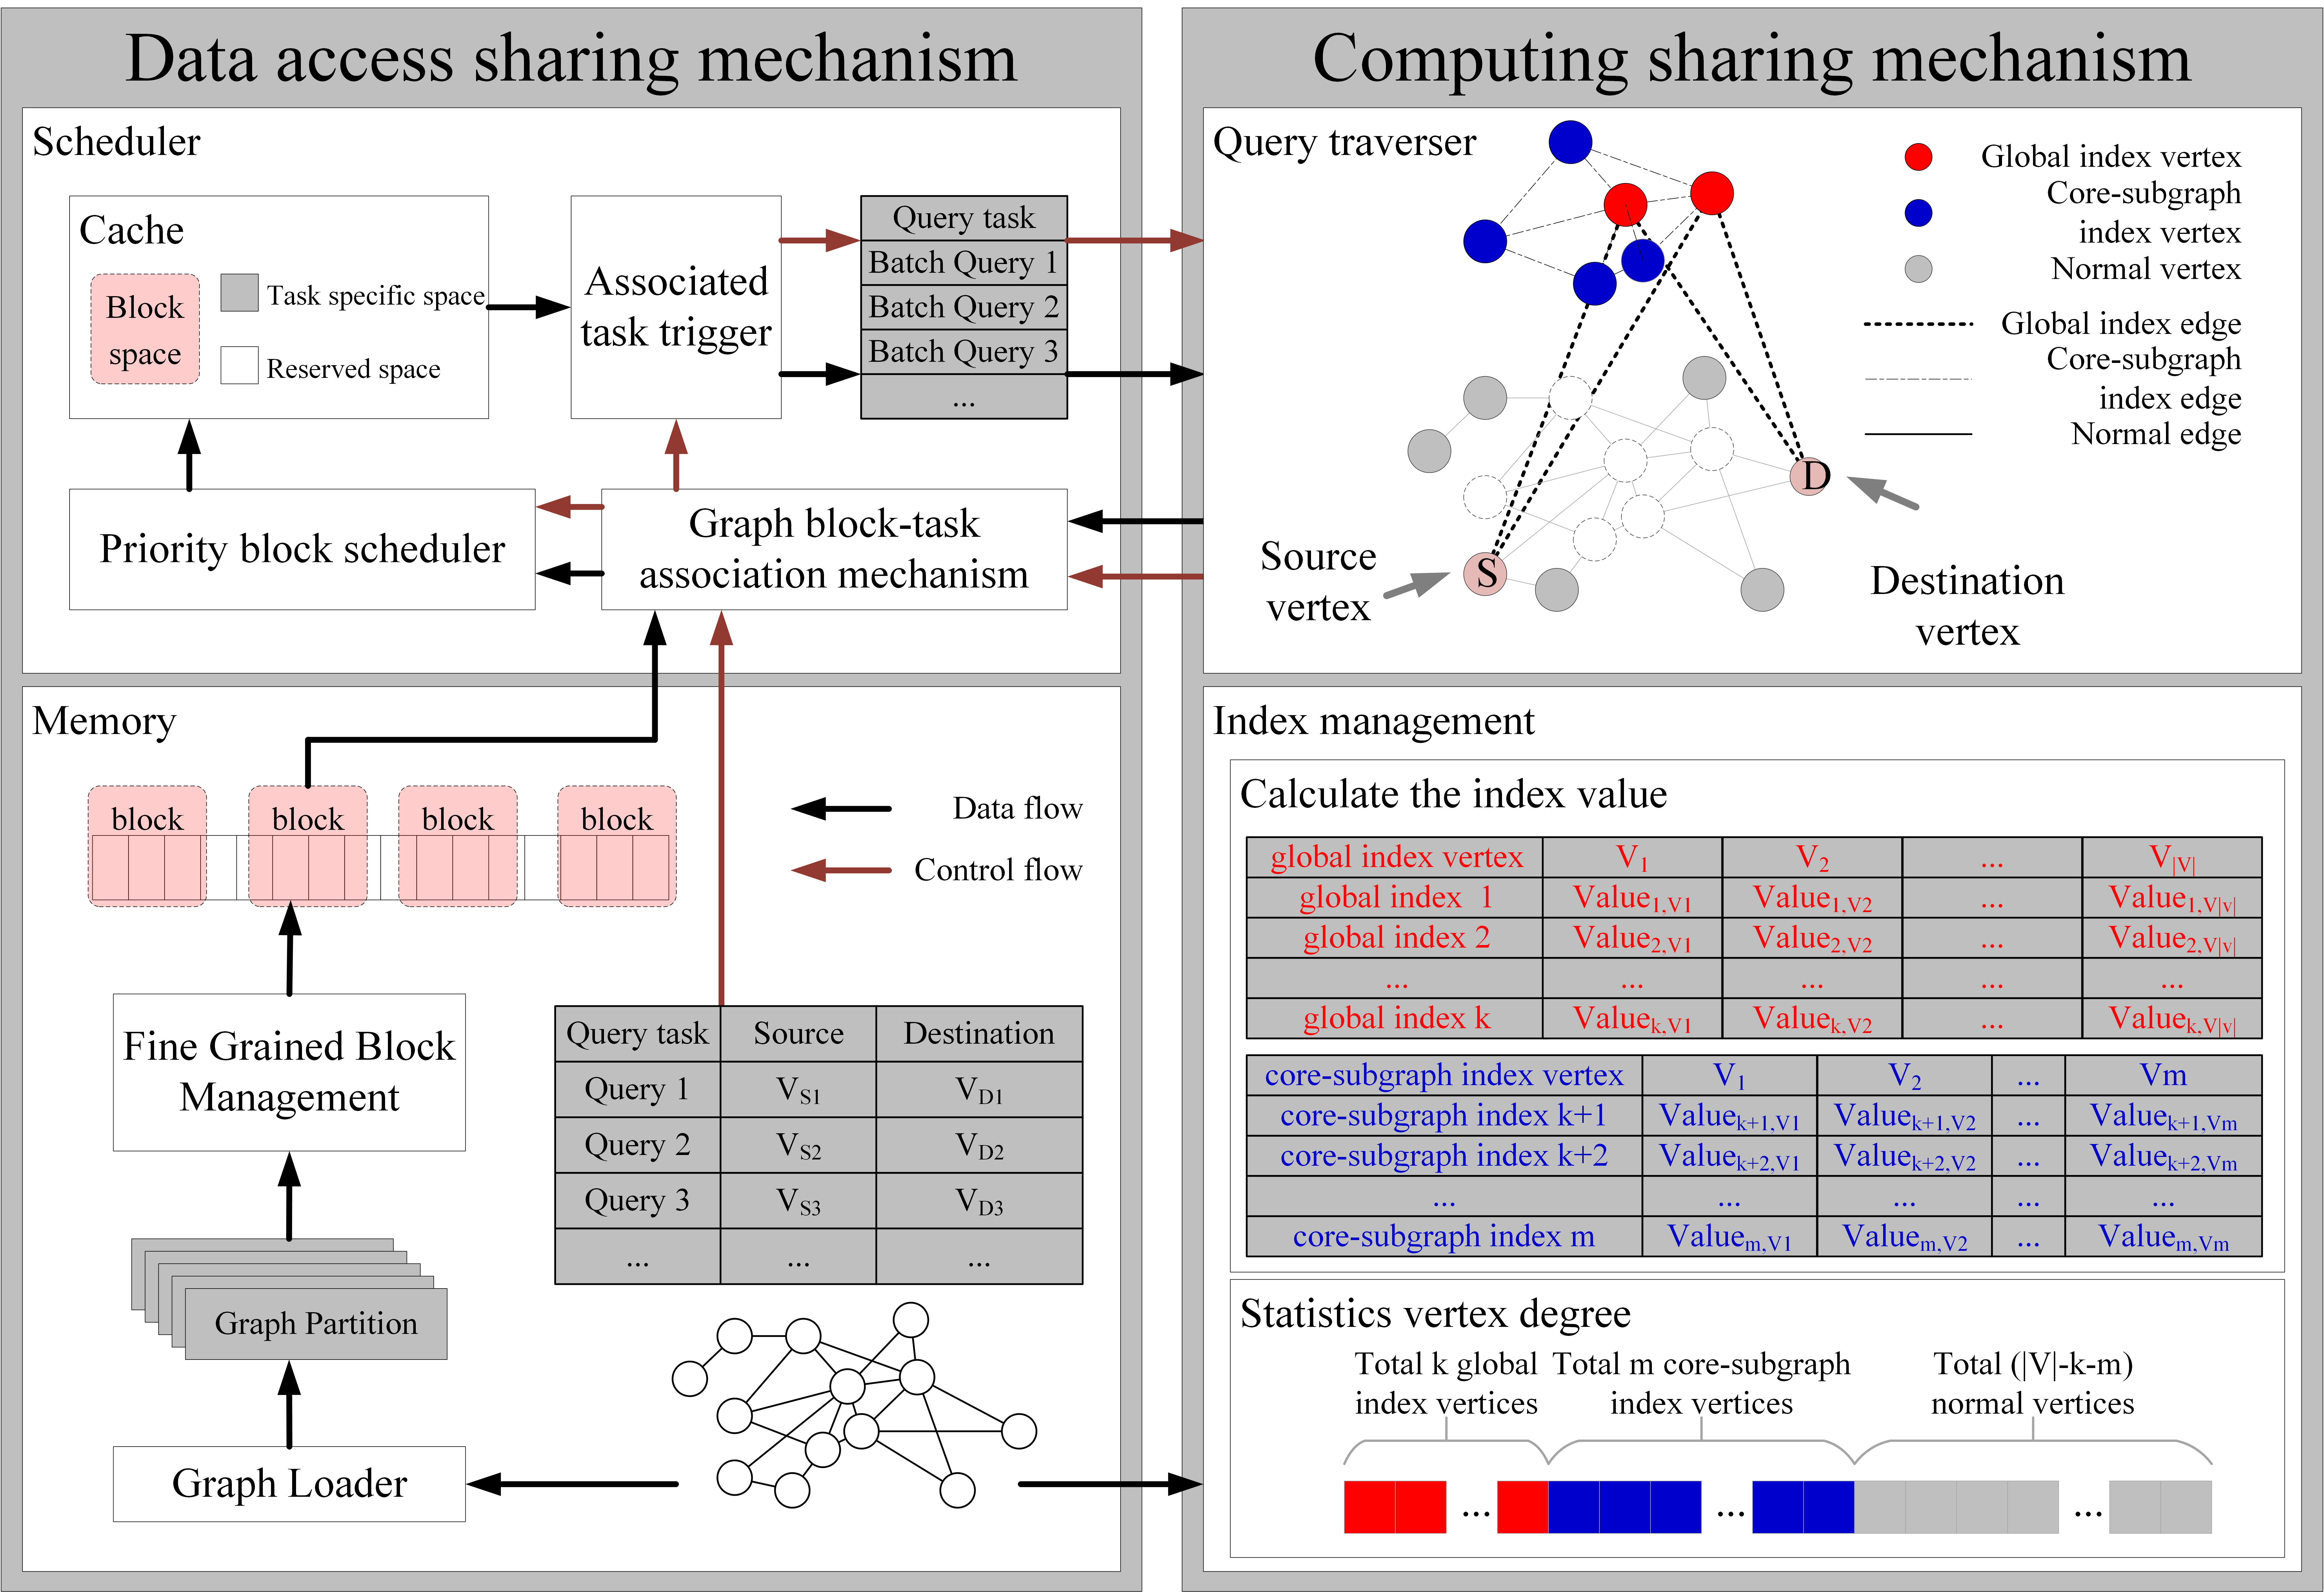
\includegraphics[width=\columnwidth]{系统架构.png}
    \caption{Your caption here}
    \label{fig:系统架构}
  \end{figure}
  

{\bf{Data Access Sharing Mechanism}}. This mechanism aims to achieve precise sharing of graph structure data by leveraging data access similarities among concurrent tasks. The process unfolds as follows: initially, similar to other distributed graph computing systems [13-16], it partitions the original graph data into coarse-grained segments, distributing them for parallel processing across different machines. Subsequently, a fine-grained chunk manager further divides these coarse-grained segments into fine-grained graph chunks. The next step involves establishing connections between query tasks and graph data chunks. Specifically, if a query task $q_i$ has active vertices in a graph chunk $b_i$, a relationship between $q_i$ and $b_i$ is established. Following this, a graph chunk priority scheduling mechanism prioritizes graph chunks with a higher number of associated tasks for loading into the Last Level Cache (LLC). Consequently, the system filters out all query tasks linked to graph chunks present in the LLC, allowing them to be executed in batches on the shared graph chunks.

{\bf{Calculation Sharing Mechanism}}. GraphCPP optimizes shared path computation by leveraging dual-level index information (global index and core subgraph index) for concurrent query tasks. The process consists of three phases: 1) Preprocessing Phase: Gather degree information for all vertices in the original graph data. Sort vertices in descending order based on degrees. Select vertices ranked from 1 to $k$ as global vertices and vertices ranked from $k+1$ to $k+m$ as core subgraph vertices. 2) Index Building Phase: Execute a point-to-all query algorithm before queries start. Compute the best path values from global vertices to all vertices in the graph (e.g., SSSP algorithm for PPSP tasks). For directed graphs, calculate outbound and inbound path values for global vertices; for undirected graphs, only one calculation is needed. Dynamically maintain the core subgraph through a runtime method. The core subgraph doesn't need precomputation for hot paths but explores them dynamically after each query, adding them to the core subgraph structure. 3) Computation Sharing Phase: Global vertices, acting as intermediaries for numerous paths, are used at the beginning of a query to compute the path value for a reachable path. This path may not be the best path but serves as a reference for pruning queries; In pruning traversal based on upper and lower bounds, the global index estimates path values for query paths earlier, enabling earlier pruning of unsuitable paths. This constitutes the first level of computation sharing; The core subgraph, maintaining best path values between hot vertices, acts as a highway network between query tasks. When a query task traverses hot vertices in the core subgraph, it connects to the highway, allowing quick traversal from entrance to exit vertices without recalculating path values. This constitutes the second level of computation sharing.


\subsection{Overall Execution Workflow}
Algorithm 1 outlines the comprehensive execution process of GraphCPP in handling concurrent query tasks. Assuming partitioning is completed, in the first line, we acquire the set \(block_{table}\), which includes all graph blocks on the current computing node, and the set \(Q\), which includes all query tasks on the current computing node. Each of them is allocated a segment of memory. In the second line, we enter a loop processing phase, and queries iterate until convergence is achieved. GraphCPP invokes \texttt{ChooseNextSharingBlock} to update the association between query tasks and graph blocks and selects the graph block \(b_i\) with the highest priority (having the most associated tasks). By tallying the associated blocks for each task (i.e., tasks with active vertices in the current block), we can determine all query tasks related to the current graph block \(b_i\) (fourth line). Next, we load \(b_i\) into the cache and parallelly process all associated query operations \(q_i\) (fifth line). This step embodies the idea of data sharing, i.e., multiple query tasks sharing the result of a single data access. Subsequently, we invoke \texttt{GraphCPPCompute} to perform point-to-point query operations \(q_i\) on the current block (details are provided in Section (section:xx)  . Iterative query task execution follows the Bulk Synchronous Parallel (BSP) model, where each iteration generates a new set of active vertices and updates to form a new query task (sixth line). If the new query remains associated with the current graph block \(b_i\), we add \(q_i\) to \(Q_{b_i}\) and return to the fifth line to continue querying on the graph block \(b_i\). Otherwise, it signifies that the new task is not associated with the current graph block, and it needs to be saved in the query task set, at this point, the task is suspended.

\begin{algorithm}
\caption{Concurrent Point-to-Point Queries}
\label{alg:concurrent_queries}
\begin{algorithmic}[1]

\Function{OverallWorkflow}{}
    \State \Call{MallocBuffers}{$block_{table}, Q$}
    \While{\Call{has\_active}{$block_{table}$}}
        \State $b_i \gets$ \Call{ChooseNextSharingBlock}{}
        \State $Q_{b_i} \gets$ \Call{ChooseAssociatedQueries}{$b_i$}
        \For{\textbf{each} $q_i \in Q_{b_i}$} 
            \State $new\_query \gets$ \Call{GraphCPPCompute}{$q_i, b_i$}
            \If{\Call{has\_Associated}{$(b_i, new\_query)$}}
                \State $Q_{b_i}.\text{Push}(new\_query)$
            \Else
                \State $Q.\text{Push}(new\_query)$
            \EndIf
        \EndFor
    \EndWhile
\EndFunction

\end{algorithmic}
\end{algorithm}
  
The presented algorithm illustrates the overall workflow of GraphCPP. In the subsequent sections, we will delve into the detailed explanations of two optimization mechanisms: data access sharing and compute sharing.

\subsection{Data Access Sharing Mechanism}
In Section 2.2, we observed a significant overlap in graph structure data access among concurrent tasks. Under the existing processing mechanism, this overlapping data cannot be shared and utilized. However, for point-to-point query tasks on the graph, the order of data access does not affect the correctness of the results. The core idea of our data sharing mechanism is to transform the original $task \rightarrow data$ linear task scheduling order into a $data \rightarrow task$ fine-grained concurrent task scheduling order. This allows us to leverage data similarity among concurrent query tasks, amortize data access overhead, enhance cache utilization efficiency, and consequently, improve system throughput. We will address two key questions in the following sections: 1) How to determine the shared data segments? 2) How to implement data sharing among multiple tasks? Finally, we will describe additional measures to further exploit data access similarity.

a) Determine Shared Data Segments

{\bf{Determine the granularity of shared graph partitions.}} Distributed memory graph computing systems need to load data into the cache to improve data access efficiency. Ideally, the data of shared graph partitions should fully fit into the Last-Level Cache (LLC) to avoid frequent eviction and reloading of different parts of partitions. However, the granularity of graph partitions should not be too small, as it would increase synchronization overhead in task processing. We use the formula x to determine an appropriate size for shared graph partitions. Here, $B_S$ repressents the size of the graph structure data for the shared partition, $G_S$ represents the size of the graph structure data for the partition it belongs to, $|V|$ is the total number of vertices on the partitioned graph, $V_S$ represents the average space required to store state information for a vertex, $N$ is the number of concurrent query tasks, $LLC_S$ is the size of the LLC cache, and $R_S$ is the size of reserved redundant space. The two terms on the right side of the formula represent graph structure data and task-specific data, respectively (their sizes are proportional to the scale of the graph partition and the number of concurrent query tasks). The right side of the formula represents the size of the available space per task after deducting the reserved cache space. Using this formula, we determine the maximum granularity for each shared graph partition under the premise of adapting to LLC capacity.

\begin{equation}
    B_S + \frac{B_S}{G_S} \cdot \lvert V \rvert \cdot V_S \cdot N \leq LLC_S - R_S
    \end{equation}

{\bf{Logical Partitioning.}} Once the granularity of shared graph blocks is established, GraphCPP can proceed with the logical partitioning during the graph preprocessing phase. This process involves subdividing coarse-grained graph partitions on the distributed system into finer-grained shared graph blocks. Pseudocode for partitioning graph blocks in GraphCPP is presented in algorithm 2:

\begin{algorithm}
\caption{Logical Partition Algorithm}
\begin{algorithmic}[1]
\Function{Partition}{$P_i, block_table$}
    \State $block\_map \gets$ null
    \For{each $e \in P_i$}
        \If{$e.src$ in $block\_map$}
            \State $block\_map[e.src] \mathrel{+{+}}$
        \Else
            \State $block\_map[e.src] \gets 1$
        \EndIf
        \If{$\text{block\_map.size()} \geq B_S$}
            \State $block_table.\text{push}(block\_map)$
            \State $block\_map.\text{clear()}$
        \EndIf
    \EndFor
\EndFunction
\end{algorithmic}
\end{algorithm}

The logical partition function takes two parameters: one is the graph partition structure data $P_i$ recorded in edge table format, and the other is the set of graph blocks $block_{table}$ owned by the partition (Line 1). In Line 2, we utilize a dictionary structure called $block_{map}$ to collect information about graph blocks. Its key records the source vertex ID of an edge, and its value records the number of outgoing edges corresponding to that vertex. In Line 4, GraphCPP iterates through each edge in the partition. If the edge has already been loaded into the current partition, the count of outgoing edges for that partition is incremented (Line 6). If the vertex is added to the dictionary for the first time, the count of outgoing edges for the partition is set to 1 (Line 8). After processing each edge, there is a check to determine if the current block is full (Line 11). If the block is full, the current block is added to the $block_{set}$ (Line 12), and the recorded block information is cleared (Line 13). This way, when all the data in the partition has been traversed, and each edge in the partition is assigned to a specific graph block, we obtain the collection of logically partitioned graph blocks.

b) Share Similar Data Among Multiple Tasks

{\bf{Establishing the Association between Shared Blocks and Query Tasks}}. Through the previous steps, we have achieved fine-grained graph partitioning in a logical manner. Since this partitioning is only logical, the data remains contiguous on the physical storage medium. Therefore, it is easy to determine the partition in which a vertex is located based on its ID. During query execution, each task $q_i$ maintains an active vertex set $Set_{act,i}$ throughout the iterative computation process. It follows the updating strategy: 1) Initially, $Set_{act,i}$ only contains the source vertex Si of the query. 2) Process the active vertices in $Set_{act,i}$ according to the flow of the point-to-point query algorithm, removing the processed vertices from the active set. 3) If a vertex's state changes in this round and it is not pruned, add the vertex to $Set_{act,i}$ for processing in the next round. We first deduce the graph block to which a vertex belongs by reverse inference of its ID and then utilize a specially designed array to store the traversed partitions for each task. Since point-to-point queries adopt a pruning-based traversal strategy, the number of active vertices in each execution round is not high. Therefore, establishing the association between query tasks and their respective blocks can be done with relatively low overhead.

{\bf{Determining the Priority of Partition Scheduling}}. After establishing the association between query tasks and their corresponding blocks, we can tally the number of tasks associated with each block. The higher the task count, the more tasks share the block, indicating greater benefits from processing this block. Consequently, blocks with a higher task count are prioritized for placement into the Last-Level Cache (LLC).

{\bf{Triggering Concurrent Execution of Associated Tasks}}. Having obtained the shared graph data blocks, based on the association between shared blocks and query tasks, we can infer the active query tasks. These tasks share the graph structure data in the LLC, and we execute these query tasks using a batch computing approach. As shown in Algorithm X, active tasks generate new active vertices after one round of execution. If these new active vertices remain associated with the current shared block, the query tasks continue execution. Shared blocks always remain in the LLC until all query tasks associated with them are processed, at which point they are evicted.

c) Batch Execute Similar Tasks

At any given moment, a diverse set of random query tasks exists in the task pool, each with distinct query paths. Tasks with high path overlap demonstrate efficient data sharing, while low overlap hinders this efficiency. Notably, we observe that higher task similarity correlates with increased path overlap, resulting in enhanced data access efficiency and reduced redundant synchronous iterations. Task similarity is quantified by calculating distance values between different task starting points (destination vertices). In GrapCPP, we propose a batch execution strategy that is aware of similar tasks, selecting batches of similar tasks from the task pool for execution. This approach further leverages data and computation similarity. Specifically, GraphCPP randomly selects a query task from the task pool, retrieves the starting and destination vertices of the task, and performs BFS algorithm to obtain the neighbor vertex sets $Set_S$ for the starting vertex and $Set_D$ for the destination vertex. Note that, considering that some central nodes may have a large number of neighbor nodes, we set an upper limit of 500 for neighbor nodes. Subsequently, it traverses the task pool, filtering out all queries with starting points in $Set_S$ and destination points in $Set_D$, treating them as similar tasks to be processed concurrently. It's important to note that if the starting or destination vertex of a query belongs to a high-degree vertex, indexing can be directly used to accelerate the query process without employing regular query steps. Excluding high-degree vertices, the overhead of the k-hop SSSP itself is minimal, and the execution process can be concurrent with regular queries, making the execution cost negligible.


\subsection{Computation Sharing Mechanism}

GraphCPP achieves computation sharing through two mechanisms: the global index and the core subgraph index. The inherent overhead of the global index is substantial and directly proportional to the number of global indices. In practice, the number of global vertices is typically kept low (e.g., 16) due to this overhead. However, because of the power-law distribution, these few hot vertices act as hub nodes for various queries. As a result, for most point-to-point queries $q_i$, a path can be traced from the source vertex $s_i$ through at least one global vertex to the destination vertex $d_i$ While this path may not always be the optimal route for $q_i$, it serves as a valuable pruning boundary. GraphCPP utilizes the global index to rapidly identify these intermediary paths, constituting the first level of computation sharing. Additionally, the core subgraph mechanism, without preprocessing, reveals optimal paths based on existing query results, facilitating computation sharing for distinct yet overlapping hot paths. Compared to the global index, the core subgraph is lighter, allowing for a broader coverage range by increasing the number of hot vertices. Consequently, more precise pruning bounds are provided, accelerating the convergence speed of pruning queries. Algorithm 3 outlines the pseudocode for the computation sharing mechanism.

\begin{algorithm}
  \caption{Shared Computation Algorithm}
  \begin{algorithmic}[1]
  
  \Function{IndexPreprocess}{$V, k, m$} 
      \State $Set_{\text{global}}, Set_{\text{core\_subgraph}} \gets \text{SortByDegree}(V, k, m)$
      \State $Set_{\text{global\_index}} \gets \text{BuildGlobalIndex}(k)$
      \State $\text{InitCoreSubgraph}(m, Set_{\text{core\_subgraph\_index}})$
  \EndFunction

  \Function{SharedComputation}{}
      \State $bound \gets \text{FirstLevelSharing}(Set_{\text{global\_index}}, Set_{\text{query}})$
      \While{$\text{activeVerticesCount} \neq 0$}
          \State $activeVertex \gets \text{GetNextActiveVertex}()$
          \If{$activeVertex \in \text{coreSubgraph}$}
              \State $\text{UpdateBounds}(bound, $\\
              $\text{SecondLevelSharing}(Set_{\text{core\_subgraph\_index}}, Set_{\text{query}}))$
          \EndIf
          \For{each $neighbor$ of $activeVertex$}
              \State $\text{UpdateBoundsByNeighbors}(neighbor)$
          \EndFor
          \State $\text{activeVerticesCount} \gets \text{UpdateActiveVertices}()$
      \EndWhile
  \EndFunction
  
  \Function{MaintainCoreSubgraph}{$Set_{\text{query\_path}}$}
      \State $Set_{\text{hot\_path}} \gets \text{ExtractHotPath}(Set_{\text{query\_path}})$
      \State $\text{AddToCoreSubgraph}(Set_{\text{hot\_path}})$
  \EndFunction

\end{algorithmic}
\end{algorithm}

The steps for implementing computation sharing are as follows:
1) Index Preprocessing (Lines 2): After sorting the degrees of vertices, the system selects the top $k+m$ hot vertices with the highest degrees. The first $k$ vertices serve as $global~vertices$ (where $k$ is user-defined), and the remaining vertices become $core~subgraph~vertices$. The computation of the global index is completed during preprocessing phrase. GraphCPP executes the SSSP algorithm to calculate the optimal paths (including index values and parent nodes) for $k$ high-degree vertices to all vertices in the graph. The results are stored in an array indexed by the high-degree vertices' IDs. The core subgraph omits the precomputation process, directly reusing the computation results of each query, requiring only initialization during preprocessing.
2) Computation Sharing (Lines 6-19): $Global~vertices$ act as pivotal nodes for query paths. Most queries have at least one path passing through global index vertices. Although this path may not be the optimal path, it provides a reliable reference for query pruning. Therefore, before executing point-to-point queries, an approximate boundary is determined using the $global~index$, representing the first level of computation sharing. Subsequently, an iterative query algorithm is executed, continuously processing new active vertices until all vertices converge. For each active vertex, it is determined whether it belongs to the core subgraph. Initially, the core subgraph is empty and does not participate in sharing. As query tasks execute, the core subgraph gradually accumulates more hot paths. When an active vertex belongs to the core subgraph, the hot path value for the corresponding starting vertex can be directly obtained through the core subgraph, avoiding redundant computation. Additionally, the core subgraph allows the query boundary to jump directly from one hot vertex to another through the hot path, accelerating the speed of point-to-point queries.
3) Maintain the Core Subgraph (Lines 20-23): To ensure the lightweight nature of the core subgraph, hot paths are not precomputed. Instead, a subset of hot paths is explored from existing optimal paths, reusing previous computation results. Clearly, any path between any two vertices on an optimal path is also an optimal path. Therefore, with minimal overhead, identifying hot vertices from existing results and calculating results between hot vertices using a prefix sum method is sufficient. To achieve this, traversal paths and path values from the source vertex to each intermediate point need to be retained during the query process. Since point-to-point queries inherently require calculating this information, the extra overhead is minimal. Through these steps, we achieve efficient data sharing using a lightweight $core~subgraph~index$.

\subsection{Update Mechanism}
In practical applications, the underlying graph traversed by query tasks often undergoes dynamic changes, involving edge additions ($e_{\text{add}}$) and edge deletions ($e_{\text{delete}}$). Changes in the graph structure data can lead to errors in index values. Therefore, when dynamic updates occur in the dynamic graph, we not only need to update the graph structure information but also dynamically update the indexes. {\bf{Graph structure information update}}: GraphCPP stores the out-neighbor of each vertex using an adjacency list. Therefore, we only need to modify the adjacency list of the corresponding out-neighbors based on the source vertex information when an edge is added (or deleted). {\bf{Index update}}: We adopt an incremental updating approach, sequentially updating the global index and core subgraph index, minimizing redundant computation costs during index updates.

The number of global index vertices is relatively small ($k$ global index vertices), but it records a substantial number of index values ($k \times |V|$ global index values). Storing these index values in a dedicated array might result in excessive bulkiness, but dispersing the index information across individual vertices is a more suitable approach. Each vertex maintains two tables: $table1$ records the parent nodes on the optimal paths to $k$ global vertices, and $table2$ records the index values of the optimal paths from this vertex to $k$ global vertices. Incremental updates are performed on these two tables based on the type of edge update. Specifically, when an edge addition update ($e_{\text{add}}$) occurs, we first obtain the source vertex $src$, destination vertex $dst$, and the weight between the two points. We then sequentially check each global index vertex. If $Index_{\text{src}} + weight > Index_{\text{dst}}$, we update $parent_{\text{dst}}$ in $table1$ to $src$ and $Index_{\text{dst}}$ in $table2$ to $Index_{\text{src}} + weight$. Otherwise, there is no need to update the index for that global vertex. In the case of an edge deletion update, we check each global index vertex and determine if $parent_{\text{dst}}$ equals $src$. If true, it indicates that we have deleted the original optimal path to $dst$, and we need to recalculate $Index_{\text{dst}}$. Similar to other incremental computation methods, updates to $dst$ will gradually propagate outward, requiring updates for all downstream vertices on the optimal paths that pass through $dst$. If $parent_{\text{dst}}$ is not equal to $src$, there is no need to update that global index vertex.

The core subgraph index records indexes between a small number of high-degree vertices, requiring the maintenance of at most $m \times m$ index values (where $m$ is orders of magnitude smaller than the graph's data scale). To store this information, we use an independent two-dimensional array for the core subgraph. Specifically, edge additions can introduce new shortcuts, leading to the degradation of original optimal paths into non-optimal ones. In the context of our pruning queries, although non-optimal path indexes can cause early overestimation of boundary values, the iterative process ensures that point-to-point queries still converge towards more optimal paths, ultimately reaching the correct optimal paths. Extracting the latest hot path values from these converged paths completes the update to hot paths. For edge deletion updates, GraphCPP checks if both vertices of the deleted edge appear on some hot path. If yes, the original hot paths are interrupted, rendering all affected hot paths invalid. If only one vertex or no vertices appear on some hot path, the deleted edge does not affect hot paths, and there is no need for an update. Since the core subgraph index reuses the optimal path results from each query, no separate calculation is needed, resulting in overall low overhead.

The above mechanism implements incremental maintenance of graph structure data, global indexes, and core subgraph indexes. Considering that subtle graph updates do not significantly impact the overall computation results, we temporarily store subtle graph updates $\Delta G$ until its size exceeds a preset threshold or a certain time interval is reached. Only then do we execute batch graph update operations, further reducing update costs.

\section{EXPERIMENTAL EVALUATION}
\subsection{Experimental Setup}

{\bf{Hardware Configuration}}: The experiments were conducted on an 8-node cluster, with each machine equipped with 2 Intel Xeon E5-2680 v4 CPUs featuring 14 physical cores, 256 GB of memory, and a 35MB Last-Level Cache (LLC). All nodes were interconnected through an Infiniband network with a bandwidth of 300Gbps. The programs were compiled using gcc version 7.5.0, openMPI version 4.1.2, and with openMP enabled.
    
{\bf{Graph Algorithms}}: To ensure alignment with previous research [xx], our study focuses on six key algorithms widely recognized as benchmarks in diverse graph-related domains, such as graph clustering, classification, and prediction. These algorithms can be classified into two categories: weighted and unweighted graph algorithms. In the realm of weighted graph algorithms, we employ Point-to-Point Shortest Path (PPSP), Point-to-Point Widest Path (PPWP), and Point-to-Point Narrowest Path (PPNP). These algorithms play a crucial role in identifying the shortest, widest, or narrowest path between two vertices, with applications ranging from social and financial networks to traffic planning, money laundering monitoring, and network quality analysis. In the category of unweighted graph algorithms, our selection includes Breadth-First Search (BFS), Connectivity, and Reachability. These algorithms address common pairwise queries on unweighted graphs, such as determining the shortest path, checking connectivity in undirected graphs, and verifying connectivity in directed graphs. Their versatility extends to advanced algorithmic applications, including bi-connectivity, higher-order connectivity, and graph clustering. This strategic choice of algorithms not only aligns with established benchmarks [xx] but also provides a comprehensive foundation for our research across various graph-related domains.

{\bf{Graph Datasets}}: The graph datasets used for the aforementioned algorithms are presented in Table x. LiveJournal and Twitter-2010 belong to social network graphs, while UK-2007-05 and Gsh-2015-host represent web-crawl graphs. These datasets exhibit power-law graphs with small diameters and skewed distributions, capturing real-world graph distribution scenarios. Our experiments are based on dynamic graphs, utilizing a snapshot mechanism where graph updates are performed on an unclosed snapshot, and graph queries are executed on a closed snapshot. Unclosed snapshots are periodically transformed into closed snapshots, replacing the original snapshot.

\begin{table}[h]
    \centering
    \begin{tabular}{lccc}
    \hline
    Datasets          & Vertices & Edges  & Data sizes \\
    \hline
    LiveJournal[1]    & 4.8M     & 69M    & 526MB      \\
    Twitter-2010[2]   & 41.7M    & 1.5B   & 10.9GB     \\
    Gsh-2015-host[3]  & 68.7M    & 1.8B   & 13.4GB     \\
    UK-2007-05[4]     & 106M     & 3.74B  & 27.9GB     \\
    \hline
    \end{tabular}
    \caption{Dataset Information}
    \end{table}

{\bf{System Comparison}}: We conducted a comparative analysis of GraphCPP's query performance with that of PnP, Tripoline, and SGraph\cite{sgraph}. Since these systems are not open source, we re-implemented their mechanisms using the Gemini distributed graph processing framework. As none of these three systems inherently supports concurrent operations, we made modifications to enable them to handle multiple jobs simultaneously. We compared the performance of these systems in two modes: PnP-S, PnP-C, Tripoline-S, Tripoline-C, SGraph-S, and SGraph-C. In systems with the ``-S" suffix, jobs are sequentially processed, while in those with the ``-C" suffix, jobs are handled concurrently, managed by the operating system.

To evaluate performance, we submitted PPsP, PPWP, PPNP, BFS, Connectivity, and Reachability queries sequentially or concurrently until a specific number of jobs were generated. Parameters for each job were set randomly, even if they belonged to the same graph algorithm. For concurrent submissions, the intervals between job submissions were also randomized. Tripoline, SGraph\cite{sgraph}, and GraphCPP employed a similar global index mechanism, with the global index set to 16 in our experiments. The core subgraph vertices in GraphCPP were set to 128. All benchmarks were executed 10 times, and the results are reported as average values.
    

\subsection{Overall Performance Comparison}

\begin{figure}[!t]
    \centering
  
    \begin{subfigure}{0.3\columnwidth}
      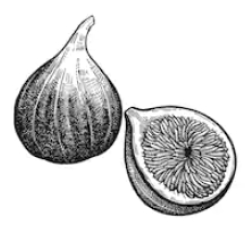
\includegraphics[width=\linewidth]{fig1.png}
      \caption{Caption for Subfigure 1}
      \label{fig:subfig1}
    \end{subfigure}
    \hfill
    \begin{subfigure}{0.3\columnwidth}
      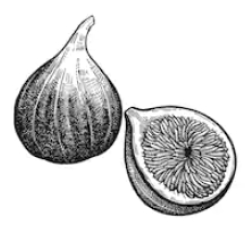
\includegraphics[width=\linewidth]{fig1.png}
      \caption{Caption for Subfigure 2}
      \label{fig:subfig2}
    \end{subfigure}
    \hfill
    \begin{subfigure}{0.3\columnwidth}
      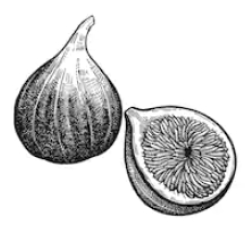
\includegraphics[width=\linewidth]{fig1.png}
      \caption{Caption for Subfigure 3}
      \label{fig:subfig3}
    \end{subfigure}
  
    \medskip
  
    \begin{subfigure}{0.3\columnwidth}
      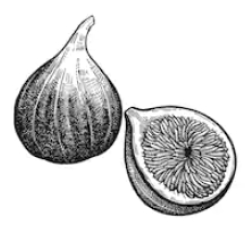
\includegraphics[width=\linewidth]{fig1.png}
      \caption{Caption for Subfigure 4}
      \label{fig:subfig4}
    \end{subfigure}
    \hfill
    \begin{subfigure}{0.3\columnwidth}
      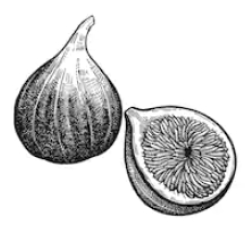
\includegraphics[width=\linewidth]{fig1.png}
      \caption{Caption for Subfigure 5}
      \label{fig:subfig5}
    \end{subfigure}
    \hfill
    \begin{subfigure}{0.3\columnwidth}
      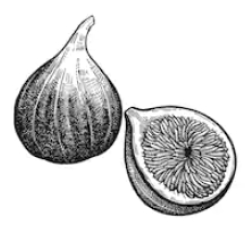
\includegraphics[width=\linewidth]{fig1.png}
      \caption{Caption for Subfigure 6}
      \label{fig:subfig6}
    \end{subfigure}
  
    \caption{Overall caption for the figure}
    \label{fig:overall}
  \end{figure}
  

Figure 9 depicts the total execution time of xx concurrent jobs using different schemes. For conciseness, only the optimal results are displayed, and due to significant variations in the execution times of different test cases, we normalize the execution time relative to PnP's performance. It is evident that, for all graphs, GraphCPP achieves shorter execution times (and higher throughput) compared to the other schemes. In comparison to SGraph-S, SGraph-C, PnP-S, PnP-C, Tripoline-S, and Tripoline-C, GraphCPP demonstrates an average throughput improvement of approximately xx, xx, xx, xx, xx, and xx times, respectively. This enhancement in throughput is accomplished by reducing data access costs and efficiently pruning the core subgraph in GraphCPP.

To provide a more in-depth analysis of performance, we further divide the total time into data access time and graph processing time. As shown in Figure 10, GraphCPP requires less time for graph data access compared to other systems, and this proportion decreases further as the graph size increases. For example, in the case of Gsh-2015-host, GraphCPP's data access time is reduced by xx times to xx times compared to other systems. Two key factors contribute to GraphCPP's efficiency: 1) identical portions of graph data required by different concurrent jobs only need to load and maintain a single copy in memory, reducing memory consumption; 2) graph data blocks are prioritized and periodically loaded into the LLC based on the number of associated tasks, promoting job reuse and effectively lowering LLC miss rates, minimizing unnecessary memory data transfers. Additionally, thanks to the two-level computing sharing mechanism, GraphCPP's computation time is also lower than that of other systems.

\subsection{Efficiency of Data Access Sharing Mechanism}
GraphCPP employs a data sharing mechanism to reduce redundant data access. To qualitatively illustrate the efficiency of this mechanism, we evaluate the LLC utilization of different systems, and the results are presented in Figure 11. Notably, GraphCPP demonstrates lower LLC miss rates compared to the other six systems. In the case of UK-2007-05, GraphCPP's LLC miss rate is only xx, while SGraph-S, SGraph-C, PnP-S, PnP-C, Tripoline-S, and Tripoline-C exhibit LLC miss rates of xx, xx, xx, xx, xx, and xx, respectively. This is primarily attributed to GraphCPP allowing multiple jobs to share a single graph data copy in the LLC, enabling more efficient utilization of the LLC and enhancing data locality for jobs.

Additionally, we track the total amount of data swapped into the LLC by these 16 jobs. Generally, the concurrent execution mode (-C) tends to swap more data into the LLC compared to the sequential execution mode (-S). This is because concurrent jobs lack data sharing, leading to frequent swapping of graph data in and out of the LLC and resulting in more redundant memory data transfers. As illustrated in Figure 12, GraphCPP swaps significantly less data compared to SGraph-S, PnP-S, and Tripoline-S (xx, xx, and xx, respectively, in UK-2007-05). This reduction is attributed to GraphCPP maximizing the similarity in data access among concurrent tasks.

\subsection{Efficiency of the Computation Sharing Mechanism}
Figure x evaluates the relationship between the processing time of each system graph and its variation over time. Due to significant differences in the graph processing time of each system, we represent the normalized time as the PnP graph processing time. PnP relies purely on pruning without utilizing an index, reducing preprocessing time but resulting in the longest query computation time. Tripoline, leveraging upper-bound pruning and a global index, reduces graph processing time. SGraph\cite{sgraph}, employing upper-bound and lower-bound pruning strategies, achieves better pruning effects, requiring fewer vertices to be computed and resulting in shorter graph processing times. While the graph processing time of these three systems may fluctuate slightly based on different query characteristics, overall, the graph processing time remains stable. In contrast, GraphCPP's graph processing time initially aligns with SGraph, as it adopts a global index mechanism similar to SGraph. However, due to the continuous improvement of GraphCPP's core subgraph index mechanism during queries, it can leverage optimizations at the second level to continuously accelerate graph processing time, resulting in a reduction over time; GraphCPP shortens its processing time.

{\bf{Global Index Overhead}}: As the number of global indices increases, the time required for maintaining the indices also grows. In our experiments, PnP did not incur maintenance overhead for global indices as it did not utilize them. However, Tripoline, SGraph\cite{sgraph}, and GraphCPP employed similar global index mechanisms. As shown in Figure x, GraphCPP's index construction overhead is comparable to other systems due to the adoption of the same number of global indices. Nevertheless, GraphCPP achieves higher throughput, allowing it to handle more queries in the same time frame, thereby distributing the global index overhead.

{\bf{Core Subgraph Index Overhead}}: We evaluated the impact of the core subgraph index on GraphCPP's performance. With the global index set to 16, GraphCPP-128, GraphCPP-256, and GraphCPP-without represent versions with core subgraph indices of 128, 256 vertices, and without using core subgraph indices, respectively. Table x illustrates the memory space occupied by these three versions of core subgraphs. It is noticeable that GraphCPP-128 and GraphCPP-256 incur only a minimal increase in memory usage compared to GraphCPP-without, all maintaining 16 global indices. This minimal increase is attributed to the fact that core subgraph vertices only store path values to other core subgraph vertices, requiring very little additional space compared to global indices storing path values to all vertices.

\begin{table}[htbp]
    \centering
    \caption{Table Title}
    \label{tab:mytable}
    \begin{tabular}{|l|c|c|}
      \hline
      & Core subgraph scale  & Total execution time \\
      \hline
      GraphCPP-without & 1 & 1 \\
      GraphCPP-128 & 1 & 1 \\
      GraphCPP-256 & 1 & 1 \\
      \hline
    \end{tabular}
  \end{table}

Moreover, Table x displays the total execution time of GraphCPP-128, GraphCPP-256, and GraphCPP-without across 16 jobs. Consistently, GraphCPP-256 and GraphCPP-128 outperform GraphCPP-without, with GraphCPP-256 being faster than GraphCPP-128. On Friendster, the processing times of GraphCPP-256 and GraphCPP-128 are only xx and xx times that of GraphCPP-without, respectively. This improvement is attributed to the additional core subgraph vertices enhancing pruning effectiveness and constraining upper and lower bounds.

{\bf{Update Maintenance Overhead}}: Tripoline, SGraph, and GraphCPP share a common global index mechanism, with an equal global index number set to 16. GraphCPP, additionally implementing a second level of sharing through the core subgraph mechanism, incurs additional maintenance overhead. As described in Section xxx, during edge addition updates, there is no need to specifically update the corresponding core subgraph hot paths. In the case of edge deletion updates, only the affected hot paths need to be deleted. Since we do not perform a dedicated computation for the core subgraph but rather extract hot paths from existing results, graph updates only affect the accuracy of the core subgraph mechanism without incurring expensive update maintenance overhead.


\subsection{Scalability of GraphCPP}
Figure 16 illustrates the performance comparison between GraphCPP and six other systems under varying numbers of concurrent PPsP jobs. GraphCPP exhibits superior performance improvement as the number of concurrent jobs increases. For 2, 4, 8, and 16 concurrent jobs, GraphCPP achieves acceleration ratios of xx, xx, xx, and xx, respectively, in comparison to SGraph-S. This improvement stems from GraphCPP's amortization, which saves more data access and storage costs with an increasing number of jobs. It's important to note that with only one concurrent job, GraphCPP's fine-grained scheduling operations do not occur, resulting in minimal differences in execution time compared to other schemes. According to our tests, the block scheduling cost of GraphCPP constitutes only xx-xx\% of the total execution time. Furthermore, due to resource contention, the performance of the concurrent version (-C) is considerably worse than both GraphCPP and the sequential version (-S). Therefore, a simple modification of existing graph processing systems to support concurrent tasks might not be an optimal choice.

Next, we assess the horizontal scalability of GraphCPP. To achieve this goal, we evaluate the performance of different schemes on 1, 2, 4, and 8 nodes. As shown in Figure 18, GraphCPP's performance on 8 nodes is xx-xx times that of a single machine, indicating robust scalability. Moreover, GraphCPP's scalability surpasses that of SGraph, PnP, and Tripoline due to lower communication costs facilitated by data sharing and core subgraph indexing. Consequently, we believe that GraphCPP can efficiently support practical point-to-point query applications.

\section{RELATED WORK}
{\bf{Graph Processing Systems}}. With the increasing prominence of graph computing as a research focus, an increasing number of diverse types of graph computing systems are being proposed. 1) Single-node in-memory graph computing systems: Ligra [x] accelerates graph computation, especially graph traversal algorithms, by switching between push and pull computation modes. KickStarter [x] and GraphBolt [x] implement incremental processing for streaming graphs. DiGraph [x] proposes an efficient iterative directed graph processing system on GPUs. LCCG [x], DepGraph [x], and TDGraph [x] utilize topology-aware execution methods, reducing redundant computation and data access costs; 2) Single-node out-of-core graph computing systems: GraphChi [x] and X-Stream [x] achieve efficient out-of-core graph processing through sequential storage access. FlashGraph [x] employs a semi-external memory graph engine, achieving high IOPS and parallelism. GridGraph [x] adopts the Streaming-Apply approach to enhance locality and reduce I/O operations. DGraph [x] accelerates graph processing through faster state propagation. GraphM [x] adopts a data-sharing approach, optimizing throughput for concurrent systems; 3) Distributed graph computing systems: Pregel [x] introduces the Bulk Synchronous Parallel (BSP) computation model, addressing the processing needs of graphs with billions of edges in terms of performance, scalability, and fault tolerance. PowerGraph [x] proposes a vertex-cut graph partitioning approach, effectively reducing communication volume and addressing load imbalance caused by high-degree vertices. PowerLyra [x] employs a hybrid computing model, using different computation strategies for high-degree and low-degree vertices. Gemini [x] introduces a dual-mode computation engine, ensuring scalability while maintaining performance. CGraph [x] uses a data-centric Load-Trigger-Pushing (LTP) model, leveraging temporal and spatial similarities between concurrent tasks to reduce distributed system overhead; The mentioned works are intended for general graph algorithms. However, point-to-point query algorithms, which concentrate on the specific relationships between vertex pairs in a graph, show notable distinctions. These query algorithms can significantly improve execution efficiency through pruning strategies. Nevertheless, general graph computing systems do not inherently accommodate such algorithms.

{\bf{Point-to-Point Queries}}. Numerous studies have been conducted on point-to-point queries. On the hardware front, $hub^2$ [x] proposed a dedicated accelerator with a hub-centric approach, accelerating the PPSP process by constraining the search scope of high-degree vertices and pruning the search process. On the software side, Quegel[x] pursued an indexing approach, enhancing query response speed by constructing a distributed static index of the graph during loading. PnP[x] took a pruning route, reducing redundant accesses and computations in point-to-point queries through a universal pruning strategy. Tripoline[x] combined both indexing and pruning, achieving incremental evaluation of queries without prior knowledge by leveraging the triangle inequality principle. SGraph[x] further optimized pruning strategies, employing upper and lower bounds to achieve sub-second latency queries on large graphs with dynamically changing data. The aforementioned efforts focus on optimizing the speed of individual point-to-point queries through mechanisms such as pruning and indexing, overlooking the substantial load posed by large-scale concurrent queries.

{\bf{Concurrent Graph Computing}}. Numerous graph computing systems have explored concurrent graph computation, especially in the realm of single-machine memory graph processing systems. For instance, Congra[x] dynamically schedules tasks based on an offline analysis of query tasks' memory bandwidth consumption and atomic operation characteristics. This dynamic scheduling aims to enhance system throughput and resource efficiency without blocking queries due to resource contention. Krill[x] introduces an SAP model that decouples graph structure, algorithms, and attributes. It simplifies attribute data management using attribute buffers and employs graph kernel fusion to reduce memory access by treating all tasks as a cohesive unit. ForkGraph[x] proposes an efficient buffer execution model for concurrent tasks, facilitating data sharing and accelerating overall execution speed through a yield-based scheduling strategy. In the context of single-machine out-of-core graph computing systems, GraphM[x] leverages the temporal and spatial locality of concurrent tasks for data sharing in concurrent graph computation. For distributed graph computing systems, Seraph[x] suggests decoupling graph structure data from task-specific data to enable concurrent tasks to share common graph structure data. MultiLyra[x] and BEAD[x] distribute communication costs among cluster computing nodes through graph and boundary sharing, supporting efficient batch query evaluations. CGraph[x] serves as the distributed version of GraphM[x]. These approaches primarily focus on optimizing data access sharing for concurrent tasks, yet they overlook computation optimization between concurrent tasks and lack specialized optimization for point-to-point queries.


\section{CONCLUSION}
Current point-to-point query systems predominantly concentrate on optimizing the speed of individual queries, overlooking the potential for throughput optimization in concurrent scenarios. This paper identifies significant data access and computation similarities among concurrent point-to-point query tasks. Introducing GraphCPP, a data-driven concurrent point-to-point query system, the paper utilizes a data-driven caching execution mechanism to achieve overlapping data access sharing among concurrent queries. Simultaneously, through a two-level computation sharing mechanism, it effectively realizes computation sharing among multiple tasks. Experimental results demonstrate that GraphCPP outperforms state-of-the-art graph query systems, such as SGraph[x], Tripoline[x], and Pnp[x], by a factor of XXX.

\section{ACKNOWLEDGMENTS}


\begin{thebibliography}{100}
  \bibliographystyle{IEEEtran}
  
  \bibitem{sgraph}
  H. Chen, M. Zhang, K. Yang, et al., ``Achieving Sub-second Pairwise Query over Evolving Graphs,'' in \textit{Proc. Int. Conf. Architectural Support Program. Languages Operating Syst.}, Vancouver, BC, Canada, 2023, pp. 1--15.
  
  \bibitem{tripoline}
  X. Jiang, C. Xu, X. Yin, et al., ``Tripoline: generalized incremental graph processing via graph triangle inequality,'' in \textit{Proc. Eur. Conf. Comput. Syst.}, United Kingdom, 2021, pp. 17--32.
  
  \bibitem{pnp}
  C. Xu, K. Vora, R. Gupta, ``Pnp: Pruning and prediction for point-to-point iterative graph analytics,'' in \textit{Proc. Int. Conf. Architectural Support Program. Languages Operating Syst.}, Providence, RI, USA, 2019, pp. 587--600.
  
  \bibitem{aligroup}
  ``Alibaba Group,'' https://www.alibabagroup.com/document-1595215205757878272, 2023.
  
  
  \bibitem{google}
  ``Google Maps,'' https://www.alibabagroup, 2023.
  
  \bibitem{facebook}
  ``Facebook,'' www.facebook.com, 2023.
  
  \bibitem{alipay}
  ``Alipay,'' www.alipay.com, 2019.
  
  \bibitem{cagis}
  ``Cagis,'' http://www.cagis.org.cn, 2021.
  
  \bibitem{baidu}
  ``Baidu Baike,'' https://baike.baidu.com, 2023.
  
  \bibitem{amap}
  ``A Map,'' https://ditu.amap.com, 2023.
  
  \bibitem{qq}
  ``Tencent Maps,'' https://map.qq.com, 2023.
  
  \bibitem{petalmaps}
  ``Petal Maps,'' https://www.petalmaps.com, 2023.
  
  \bibitem{gemini}
  X. Zhu, W. Chen, W. Zheng, et al., ``Gemini: A {Computation-Centric} Distributed Graph Processing System,'' in \textit{USENIX Symp. Operating Syst. Des. Implementation}, Savannah, GA, USA, 2016, pp. 301--316.
  
  \bibitem{giraph}
  C. Avery, ``Giraph: Large-scale graph processing infrastructure on hadoop,'' in \textit{Proc. Hadoop Summit}, pp. 5--9, 2011.
  
  \bibitem{graphlab}
  Y. Low, J. Gonzalez, A. Kyrola, et al., ``Graphlab: A new framework for parallel machine learning,'' \textit{arXiv preprint arXiv:1408.2041}, 2019.
  
  \bibitem{powergraph}
  J. Gonzalez, Y. Low, H. Gu, et al., ``{PowerGraph}: Distributed {Graph-Parallel} Computation on Natural Graphs,'' in \textit{USENIX Symp. Operating Syst. Des. Implementation}, Hollywood, CA, USA, 2012, pp. 17--30.
  
  \bibitem{graphx}
  J. Gonzalez, R. Xin, A. Dave, et al., ``{GraphX}: Graph Processing in a Distributed Dataflow Framework,'' in \textit{USENIX Symp. Operating Syst. Des. Implementation}, Broomfield, CO, USA, 2014, pp. 599--613.
  
  \bibitem{soa}
  C. Xie, R. Chen, H. Guan, et al., ``Sync or async: Time to fuse for distributed graph-parallel computation,'' \textit{ACM SIGPLAN Notices}, vol. 50, no. 8, pp. 194--204, 2015.
  
  \bibitem{powerlyra}
  R. Chen, J. Shi, Y. Chen, et al., ``Powerlyra: Differentiated graph computation and partitioning on skewed graphs,'' \textit{ACM Trans. Parallel Comput.}, vol. 5, no. 3, pp. 1--39, 2019.
  
  \bibitem{snap}
  ``Stanford large network dataset collection,'' http://snap.stanford.edu/data/index.html, 2020.
  
  \bibitem{twitter}
  H. Kwak, C. Lee, H. Park, et al., ``What is Twitter, a social network or a news media?'' in \textit{Proc. Int. Conf. World Wide Web}, Raleigh, NC, USA, 2020, pp. 591--600.
  
  \bibitem{bubing}
  P. Boldi, A. Marino and M. Santini, et al.,  ``BUbiNG: Massive Crawling for the Masses,''  \textit{ACM Trans. Web}, vol. 12, no. 2, pp. 1--26, 2018.
  
  \bibitem{timeaware}
  P. Boldi, M. Santini and S. Vigna,  ``A large time-aware web graph,''  \textit{ACM SIGIR Forum}, vol. 42, no. 2, pp. 33--38, 2008.
  
  \bibitem{ligra}
  J. Shun, J. Blelloch, ``Ligra: a lightweight graph processing framework for shared memory,'' in \textit{Proc. Symp. Princ. Pract. Parallel Program.}, Shenzhen, China, 2013, pp. 135--146.
  
  \bibitem{kickstarter}
  K. Vora, R. Gupta, G. Xu, ``Kickstarter: Fast and accurate computations on streaming graphs via trimmed approximations,'' in \textit{Proc. Int. Conf. Architectural Support Program. Languages Operating Syst.}, New York, NY, USA, 2017, pp. 237--251.
  
  \bibitem{graphbolt}
  M. Mariappan, K. Vora, ``Graphbolt: Dependency-driven synchronous processing of streaming graphs,'' in \textit{Proc. EuroSys Conf.}, Dresden , Germany, 2019, pp. 1--16.
  
  \bibitem{digraph}
  Y. Zhang, X. Liao, H. Jin, et al., ``DiGraph: An efficient path-based iterative directed graph processing system on multiple GPUs,'' in \textit{Proc. Int. Cinf. Architectural Support Program. Languages and Operating Syst.}, Providence, RI, USA, 2019, pp. 601--614.
  
  \bibitem{lccg}
  J. Zhao, Y. Zhang, X. Liao, et al., ``LCCG: A Locality-Centric Hardware Accelerator for High Throughput of Concurrent Graph Processing,'' in \textit{Int. Conf. High Perform. Comput., Netw., Storage Anal.}, New York, NY, USA, 2021, pp. 1--14.
  
  \bibitem{depgraph}
  Y. Zhang, X. Liao, H. Jin, et al., ``DepGraph: A Dependency-Driven Accelerator for Efficient Iterative Graph Processing,'' in \textit{IEEE Int. Symp. High-Perform. Comput. Architecture }, Seoul, Korea, 2021, pp. 371--384.
  
  \bibitem{tdgraph}
  J. Zhao, Y. Yang, Y. Zhang, et al., ``TDGraph: a topology-driven accelerator for high-performance streaming graph processing,'' in \textit{Proc. Annu. Int. Symp. Comput. Architecture}, New York, NY, USA, 2022, pp. 116--129.
  
  \bibitem{graphchi}
  A. Kyrola, G. Blelloch, C. Guestrin, ``{GraphChi}:{Large-Scale} Graph Computation on Just a {PC},'' in \textit{Proc. USENIX Symp. Operating Syst. Des. Implementation}, Hollywood, CA, USA, 2012, pp. 31--46.
  
  \bibitem{x-stream}
  A. Roy, I. Mihailovic, W. Zwaenepoel,  ``X-stream: Edge-centric graph processing using streaming partitions,'' in \textit{Proc. ACM Symp. Operating Syst. Princ.}, Farminton, Pennsylvania, USA, 2013, pp. 472--488.
  
  \bibitem{flashgraph}
  D. Zheng, M. Mhembere, R. Burns, et al., ``{FlashGraph}: Processing {Billion-Node} Graphs on an Array of Commodity {SSDs},'' in \textit{USENIX Conf. File Storage Technologies}, Santa Clara, CA, USA, 2015, pp. 45--58.
  
  \bibitem{gridgraph}
  X. Zhu, W. Han, W. Chen, ``{GridGraph}:{Large-Scale} Graph Processing on a Single Machine Using 2-Level Hierarchical Partitioning,'' in \textit{USENIX Annu. Tech. Conf.}, Santa Clara, CA, USA, 2015, pp. 375--386.
  
  \bibitem{efficient}
  Y. Zhang, X. Liao, X. Shi, et al., ``Efficient Disk-Based Directed Graph Processing: A Strongly Connected Component Approach,'' \textit{IEEE Trans. Parallel Distrib. Syst.}, vol. 29, no. 4, pp. 830--842, 2018.
  
  \bibitem{graphm}
  J. Zhao, Y. Zhang, X. Liao, et al., ``GraphM: an efficient storage system for high throughput of concurrent graph processing,'' in \textit{Proc. Int. Conf. High Perform. Comput., Netw., Storage and Anal.}, Denver, Colorado, USA, 2019, pp. 1--14.
  
  \bibitem{pregel}
  G. Malewicz, M. Austern, A. Bik, et al., ``Pregel: a system for large-scale graph processing,'' in \textit{Proc. ACM SIGMOD Int. Conf. Manage. Data}, New York, NY, USA, 2010, pp. 135--146.
  
  \bibitem{cgraph}
  Y. Zhang, J. Zhao, X. Liao, et al., ``{CGraph}: A Correlations-aware Approach for Efficient Concurrent Iterative Graph Processing,'' in \textit{USENIX Annu. Tech. Conf.}, Boston, MA, USA, 2018, pp. 441--452.
  
  \bibitem{hub}
  R. Jin, N. Ruan, B. You, et al., ``Hub-accelerator: Fast and exact shortest path computation in large social networks,'' \textit{arXiv preprint arXiv:1305.0507}, 2013.
  
  \bibitem{quegel}
  Q. Zhang, D. Yan and J. Cheng, ``Quegel: A general-purpose system for querying big graphs,'' in \textit{Proc. Int. Conf. Manage. Data}, New York, NY, USA, 2016, pp. 2189--2192.
  
  \bibitem{Congra}
  P. Pan and C. Li, ``Congra: Towards Efficient Processing of Concurrent Graph Queries on Shared-Memory Machines,'' in \textit{IEEE Int. Conf. Comput. Des.}, Boston, MA, USA, 2017, pp. 217--224.
  
  \bibitem{krill}
  H. Chen, M. Shen, N. Xiao, et al., ``Krill: a compiler and runtime system for concurrent graph processing,'' in \textit{Proc. Int. Conf. High Perform. Comput., Netw., Storage and Anal.}, New York, NY, USA, 2021, pp. 1--16.
  
  \bibitem{cache}
  S. Lu, S. Sun, J. Paul, et al., ``Cache-efficient fork-processing patterns on large graphs,'' in \textit{Proc. Int. Conf. Manage. Data}, New York, NY, USA, 2021, pp. 1208--1221.
  
  \bibitem{seraph}
  J. Xue, Z. Yang, Z. Qu, et al., ``Seraph: an efficient, low-cost system for concurrent graph processing,'' in \textit{Proc. Int. Symp. High-perform. Parallel Distrib. Comput.}, Vancouver, BC, Canada, 2014, pp. 227--238.
  
  \bibitem{multilyra}
  A. Mazloumi, X. Jiang, R. Gupta, ``Multilyra: Scalable distributed evaluation of batches of iterative graph queries,'' in \textit{IEEE Int. Conf. Big Data}, Los Angeles, CA, USA, 2019, pp. 349--358.
  
  \bibitem{bead}
  A. Mazloumi, C. Xu, Z. Zhao, et al., ``BEAD: Batched Evaluation of Iterative Graph Queries with Evolving Analytics Demands,'' in \textit{IEEE Int. Conf. Big Data}, 2020, pp. 461--468.
  
  
  
  
  \end{thebibliography}

\begin{IEEEbiographynophoto}{Jane Doe} %这里的Jane Doe是指作者的名字
Biography text here without a photo.
\end{IEEEbiographynophoto} %这个是作者的结束

\begin{IEEEbiography}[{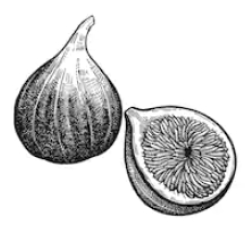
\includegraphics[width=1in,height=1.25in,clip,keepaspectratio]{fig1.png}}]{IEEE Publications Technology Team}
In this paragraph you can place your educational, professional background and research and other interests.\end{IEEEbiography} %这行的作用是插入作者的照片


\end{document}


